\label{chap6}
To be able to evaluate the proposed solution in a real-life scenario, a prototype based on the concept presented was built. This chapter introduces the implementation from a high level
view, followed by the evaluation of the result. Afterwards, the results are discussed and improvements are suggested.
\section{Implementation}

\subsection{Bus interface}
The necessary software, running on each platform, is written in the programming language "C". To interface with \gls{knx}, an \gls{api} named \gls{eibd} is used, providing functions to
send \gls{knx} frames to and receive frames from the bus. \gls{eibd} offers synchronous as well as asynchronous calls for sending and receiving frames. While the first kind of
call will block until the operation finished, the second kind of call will return immediately, the status of such calls can be checked by another special \gls{eibd} call.
Because it is not possible to use callbacks with asynchronous calls, the implementation uses the synchronous functions.

\subsubsection{Reading frames from the bus}
\gls{eibd} provides a function to monitor the bus, this way all frames are available to the application.

\begin{lstlisting}[style=cStyle,caption={Reading \gls{knx} frames},label=lst:busMon]
EIBConnection *fd;
fd = EIBSocketURL(socketPath);
EIBOpenVBusmonitor(fd);
len = EIBGetBusmonitorPacket (fd, BUFSIZE, buffer);
\end{lstlisting}

\subsubsection{Writing frames to the bus}
To write frames to the bus \gls{eibd} offers distinct functions for addressing individual devices or all devices in the segment. A connection must be first by calling the corresponding
function, afterwards the data can be written to the bus:

\begin{lstlisting}[style=cStyle,caption={Writing to \gls{knx} frames},label=lst:knxWrite]
// open an individual connection
EIBOpenT_Individual(fd, destination, 0);
// or a broadcast connection
EIBOpenT_Broadcast(fd, 0);
// finally, send the data
EIBSendAPDU(fd, len, (const uint8_t *)buf);
\end{lstlisting}

\subsubsection{KNX addressing scheme}

Care must be taken that no duplicate \gls{knx} addresses are used within the network. Therefore, the following addressing convention is proposed:
While it would be possible to use the same addresses on both lines per gateway, a different scheme is proposed.
For the secured network, the address ranges starting at address 1.1.1 to address 1.1.15 and 1.2.1 to 1.2.15 are reserved for secure line number
1 and 2 respectively, which allows a maximum of 15 gateways. Different addresses are used mainly because it facilitates debugging. 
On the unsecured lines, every gateway uses an address from the range 1.0.1 - 1.0.15. Addresses are assigned in a linearly ascending way, so gateway number 1
uses addresses 1.1.1 and 1.2.1 for secure lines 1 and 2, and 1.0.1 for its unsecured line.

\subsection{Concurrency}
Every platform possesses three distinct interfaces to the bus (two interfaces form the redundant "secure" part of the network, one is connected
to a standard \gls{knx} network), so care must be taken that no frames are missed or delayed due to a blocking call to \gls{eibd}. This can be achieved by splitting the main program into different 
processes or alternatively, threads, where for each critical task, a distinct part is responsible. While threads share the same address space, facilitating communication with
each other, processes rely on special system calls 
to share information. Additionally, thread-creation and switching between threads consumes less computing resources. Therefore, it was decided to choose the multi-threaded
approach. Consequently, at least three different threads - one for each communication interface - are needed. Nevertheless, because every thread must be able to write to or receive
frames from the bus at unpredictable moments, seven different threads are used: the main thread only handles argument processing and creates the other threads. For the remaining threads,
two pairs are responsible for the interfaces to the secured network, while the remaining thread pair interfaces to the unsecured part of the network. This setup is shown in
Figure \ref{fig:Concthreads}.
\begin{figure}[h]
\centering
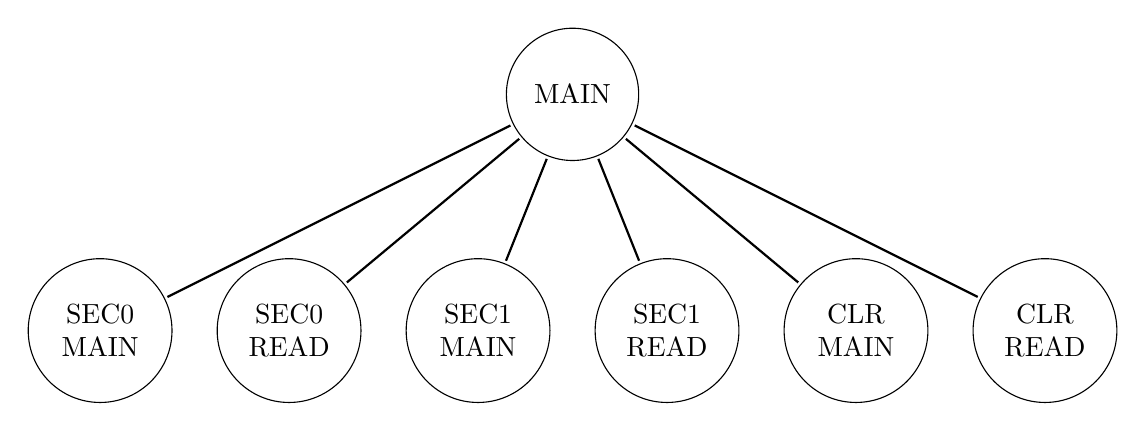
\begin{tikzpicture}[scale=0.2]
\tikzstyle{every node}+=[inner sep=2pt]
\tikzstyle{arrow}=[draw, -latex] 
\tikzset{
    pil/.style={
           ->,
           thick,
           shorten <=1pt,
           shorten >=1pt,}
}
\usetikzlibrary{automata,positioning}
\usetikzlibrary{positioning}
\node[state,text width=1.5cm,align=center]					at (-10,5)		(m)			{MAIN}; 
\node[state,text width=1.5cm,align=center]					at (-40,-10)	(sec0m)	{SEC0 MAIN}; 
\node[state,text width=1.5cm,align=center]					at (-28,-10)	(sec0r)		{SEC0 READ}; 
\node[state,text width=1.5cm,align=center]					at (-16,-10)	(sec1m)	{SEC1 MAIN}; 
\node[state,text width=1.5cm,align=center]					at (-4,-10)		(sec1r)		{SEC1 READ}; 
\node[state,text width=1.5cm,align=center]					at (8,-10)	(clrm)		{CLR MAIN}; 
\node[state,text width=1.5cm,align=center]					at (20,-10)	(clrr)			{CLR READ};
\path[pil,-] (m)  edge[auto]   node[] {} (sec0m); 
\path[pil,-] (m)  edge[auto]   node[] {} (sec0r); 
\path[pil,-] (m)  edge[auto]   node[] {} (sec1m); 
\path[pil,-] (m)  edge[auto]   node[] {} (sec1r); 
\path[pil,-] (m)  edge[auto]   node[] {} (clrm); 
\path[pil,-] (m)  edge[auto]   node[] {} (clrr); 

%\path[pil,->] (sec0r)  edge[auto, out=240, in=300]   node[] {} (sec0m); 
%\path[pil,->] (sec1r)  edge[auto, out=240, in=300]   node[] {} (sec1m); 
%\path[pil,->] (clrr)  edge[auto, out=210, in=290]   node[] {} (sec1m); 
%\path[pil,->] (clrr)  edge[auto, out=230, in= 180]   node[] {} (sec0m); 
\end{tikzpicture}
\caption{Threads used in the implementation}
\label{fig:Concthreads}
\end{figure}
This design allows to assign one timing-critical task to every thread: every READ thread immediately opens its corresponding bus interface in "monitor" mode, allowing it
to read all the bus traffic on the corresponding line. After that, it enters a loop, performing a blocking read call to \gls{eibd} on every iteration.
This will set the whole thread to "blocked", and the operating
system will set another thread or process as runnable. Whenever data is available to the blocked thread, the operating system will buffer the received data and eventually set the
thread runnable again. Thus, no frames will be missed.
\\
\\
The main-threads of the secure lines (i.e., SEC0 MAIN and SEC1 MAIN) will start the synchronization sequence, as described in Section \ref{syncService}, and send out
the synchronization messages. After  that, the main threads will enter the READY state and listen for discovery messages.
\\
\\
Whenever the CLR READ thread receives new data, the frame will be forwarded to both SEC MAIN threads together with the counter for the unique source address, contained
in the frame. Both SEC MAIN threads will send discovery requests, independently from each other, each containing newly chosen \gls{ecdh} parameters. Responsible gateways (i.e.,
gateways which are connected to the wanted destination address through their cleartext lines) will compute a new \gls{ecdh} parameter, derive distinct shared secrets for both lines,
save them and send the parameters contained in the discovery responses back to the requesting device. The requester than derives the same shared secrets, and sends the encrypted frame,
contained in extended \gls{knx} frames, to the destination gateways, which will check and decrypt them and forward both decrypted frames and the corresponding global counter values
to the CLR MAIN thread. Here, the duplicate will be discarded and one frame will be sent to its final destination.
\\
\\
A thread can be created in C with the function \textit{pthread\_create()}. The function expects four parameters:
\begin{itemize}
 \item a variable of type \textit{pthread\_t}
 \item attributes for the new thread, or NULL for default values
 \item a function pointer, serving as entry-point for the new thread
 \item parameters for the function pointer, or NULL
\end{itemize}
\begin{lstlisting}[style=cStyle,caption={Creating a new thread},label=lst:pthread_create]
if((pthread_create(&sec1MasterThread, NULL, (void *)secMasterStart, &threadEnvSec[0])) != 0)
{
  printf("sec1Thread thread init failed, exit\n");
  return -1;
}
\end{lstlisting}
If the call to \textit{pthread\_create()} succeeds, the new thread will start executing the function provided via the function pointer, and the main thread which called 
\textit{pthread\_create()} will continue. Which of the threads is running first and in which order the threads are assigned to the processor is unknown and determined by the operating
system.

\subsection{Thread-to-thread communication}
To pass data from one thread to another, different ways are possible. While the easiest way would be to use global data structures, the implementation uses 
\gls{posix}-pipes instead, mainly because with pipes, timeouts can be implemented easily. Such timeouts are used when waiting for synchronization replies, as well as for 
cleanup tasks.
\\
How to create a new pipe is shown in Listing \ref{lst:pipe}.
\begin{lstlisting}[style=cStyle, caption={Creating a pipe},label=lst:pipe]
int pipefd[2];
if(pipe(pipefd) == -1)
{
  printf("pipe() failed, exit\n");
  exit(-1);
}
\end{lstlisting}
Every pipe possesses two file descriptors, providing a uni-directional data channel: data can be written to the pipe by performing a write() - operation to the \textit{write}-end of the
pipe (index 1), while the data can be read from the pipe by calling read() with the \textit{read}-end of the pipe (index 0). Basically, the read() operation will block until new data can be read - in 
combination with the select() system call, a maximum time for the blocking operation can be set, as shown in Listing \ref{lst:timeout}.
\begin{lstlisting}[style=cStyle,caption={Blocking read with timeout},label=lst:timeout]
fd_set set;
struct timeval timeout;
int selectRC;
...
FD_ZERO(&set);
FD_SET(fileDescriptor, &set);
timeout.tv_sec = 2;	// set timeout to 2 seconds
timeout.tv_usec = 0;
selectRC = select(FD_SETSIZE, set, NULL, NULL, timeout);
if(selectRC == 0)
{
   // timeout occured
}
else if(selectRC < 0)
{
  // error occured
}
else
{
  // data arrived - read it:
  read(pipefd[READEND], buffer, len);
}
\end{lstlisting}
In this example, FD\_ZERO at first clears the set containing the file handles to be watched, FD\_SET() then adds the file handle we are interested in (allowing to watch multiple file
descriptors). The timeout is then set to two seconds 
(microseconds granularity is supported, nevertheless the timing precision is limited by the system clock granularity and kernel scheduling delays), and select() is called. If no data is
received within 2 seconds, the if-branch is executed. If data is received in time, the else-branch is executed instead, and the waiting data can be obtained by performing a standard
read() call.

\subsection{Race conditions}
Software race conditions occur whenever an application, using shared resources, depends on the timing of its processes or threads.
Because the exact time when a particular process or thread is scheduled by the processor is unknown in advance, such conditions must be avoided.
An example of a program containing a race condition would be as following:
\begin{lstlisting}[style=cStyle,caption={Race condition},label=lst:raceCond]
for ( int i = 0; i < 1000000; i++ )
{
   x = x + 1; 
}
// x = ?
\end{lstlisting}
For a single-threaded program, this would produce the value $x=1000000$ after the loop, while for a 2-threaded program, the resulting value will depend on the exact scheduling of the
threads and very likely differ from the expected value $x=2000000$. The reason is that the statement incrementing x is no atomic operation. Instead, the operation will consist of
several statements on machine language level, forming a \textit{critical region}:
\begin{enumerate}
 \item load value from address into register
 \item add 0x01 to the register
 \item write value from register to address
\end{enumerate}
If thread 1 gets interrupted after the second step and thread 2 afterwards finishes, thread 1 will overwrite the value just written by thread 2 and thus produce a false result.
\\
\\
Such a critical region must be protected such that only one thread can enter it, a requirement also called mutex, short for \textit{mut}ual \textit{ex}clusion.
The implementation uses the \gls{posix} \textit{pthread mutex} to lock critical regions, as shown in Listing \ref{lst:mutex}.  
\begin{lstlisting}[style=cStyle,caption={Locking a critical region},label=lst:mutex]
if(pthread_mutex_init(&globalMutex, NULL) != 0)
{
  printf("mutex init failed, exit");
  return -1;
}
pthread_mutex_lock(&globalMutex);
/*
    CRITICAL REGION
*/
pthread_mutex_unlock(&globalMutex);
\end{lstlisting}
\textit{globalMutex} is a global variable of type \textit{pthread\_mutex\_t}, shared between all threads which are accessing the shared resource. After calling pthread\_mutex\_lock(),
there are two possibilities: if the mutex is unlocked, the call will lock it and continue the program flow. If it is already locked, the call to pthread\_mutex\_lock() will block and
the corresponding thread will be set to blocking.
If the mutex is unlocked by the possessing thread, the blocked thread will be set active, lock for his part and continue execution.\footnote{Of course, pthread\_mutex\_lock() must
be executed in an atomic way, otherwise introducing a race condition on another level.}
\\
\\
Communication between the CLR and SEC0/SEC1 threads is achieved by pipes, as introduced above. Because data exchanged by pipes does not possess any internal structure, accessing
them must be done in a consistent way, which is the task of \textit{globalMutex}. If one thread wants to write data to another thread, it first locks the mutex, writes the
data to the pipe and finally releases the mutex. The reading thread, waiting for data in state "blocked", will be set running by the operating system, immediately lock the mutex
and read the data. Finally, it will unlock the mutex again.

\subsection{Cryptographic functions}
To use the needed cryptographic functions, the open source library "OpenSSL" is utilized. The \gls{api} supports a wide range of symmetric and asymmetric encryption, 
decryption, signing and key negotiation algorithms through two different kind of interfaces: a high level "EVP" interface, hiding much of the complexity, and 
a low level interface. If possible, the high level interface should be used, but for the key derivation function it turned out that the low level interface was easier to use.
\\
\\
Documentation and code snippets can be found on https://wiki.openssl.org, another important source of information are the man-pages (available under Debian after installing the
package libssl-doc) and the header files.
\\
\\
It is noted that in the examples below no error checking of the return codes returned by the OpenSSL calls is executed. These checks are omitted here just for clarity, nevertheless it is
imperative to always check for error conditions.

\subsubsection{Key derivation}
To obtain a shared secret between two security gateways, \gls{ecdh} over the curve
"NID X9 62 prime256v1" is used. This is a \gls{nist} elliptic curve defined over the 256 bit prime
$p_{256} = 2^{256} - 2^{224} + 2^{192} + 2^{96} - 1$, thus the resulting points will have coordinates of size 256 bits each. The uncompressed form of such a point consists of 65
bytes: 1 byte for a leading tag, 32 bytes for the x and 32 bytes for the y coordinate of the point. Because of the quadratic form of the curve (see Section \ref{sec:ecIntro} for a recap),
it suffices to transmit only the x coordinate and one byte, determining the sign of the solution. The corresponding y coordinate can than be recovered.
\\
\\
Whenever a security gateway receives a new frame on its cleartext line, it generates a new \gls{ecdh} parameter, i.e., it generates a new key pair, the public key is then sent to all
other security gateways in the segment:
\begin{lstlisting}[style=cStyle,caption={Generating an \gls{ecdh} parameter},label=lst:genEC]
EC_KEY *pkey;
pkey = EC_KEY_new_by_curve_name(NID_X9_62_prime256v1)
EC_POINT *ecPoint = NULL;
size_t ecPoint_size;
const EC_GROUP *group;
EC_KEY_generate_key(pkey));
EC_KEY_set_conv_form(pkey, POINT_CONVERSION_COMPRESSED);
ecPoint = (EC_POINT *) EC_KEY_get0_public_key(pkey);
group = (EC_GROUP *)EC_KEY_get0_group(pkey);
ecPoint_size = EC_POINT_point2oct(group, ecPoint, EC_KEY_get_conv_form(pkey), buf, BUFSIZE, NULL);
if(!EC_POINT_is_on_curve(group, ecPoint, NULL))
{
  printf("ERROR: point not on curve\n");
  exit(-1);
}
\end{lstlisting}
The new key pair is generated in line 6, the public key is obtained and converted to a hexadecimal string in lines 8 and 10. Finally, it is checked if the new point indeed is part of
the curve.
\\
\\
The receiving side performs the same operations to obtain its own key pair which is sent back to the requester, and immediately derives the shared secret
as shown in Listing \ref{lst:derive}.

\begin{lstlisting}[style=cStyle,caption={Deriving a shared secret},label=lst:derive]
size_t secret_len;
unsigned char *secret;
EC_POINT *peerEcPoint = NULL;
EC_KEY *peerEcKey = NULL;
const EC_GROUP *group = NULL;
peerEcKey = EC_KEY_new_by_curve_name(NID_X9_62_prime256v1);       
group = EC_KEY_get0_group(peerEcKey);
peerEcPoint = EC_POINT_new(group);
EC_POINT_oct2point(group, peerEcPoint, peerPubKey, (size_t)33, NULL))
EC_KEY_set_public_key(peerEcKey, peerEcPoint))
secret = OPENSSL_malloc(32);
secret_len = ECDH_compute_key(secret, 32, EC_KEY_get0_public_key(peerEcKey), pkey, NULL);
\end{lstlisting}
Here, the public key received (the pointer \textit{peerPubKey}) must be first converted from a hexadecimal string into point representation, and finally into an EC\_KEY object
(lines 9 and 10). The actual key derivation is shown in line 12.
\\
\\
This derived secret must be fed into a secure hashing function, for example \gls{sha}-256 because the shared secret may not be uniformly distributed. By appending different strings
it is also possible to derive an encryption and a \gls{mac2} key in one run.

\subsubsection{MAC generation}
For this task, a \gls{sha}-256 based \gls{hmac} is used, producing a 32 byte \gls{mac2}. To reduce the overhead, only 4 bytes are used and contained in the messages. The usage of
the high-level \gls{api} is shown in Listing \ref{lst:hmac}.
\begin{lstlisting}[style=cStyle,caption={Generating an \gls{hmac}},label=lst:hmac]
size_t req = 0;
EVP_MD_CTX* ctx = EVP_MD_CTX_create();
const EVP_MD* md = EVP_get_digestbyname("SHA256");
EVP_DigestInit_ex(ctx, md, NULL);
EVP_DigestSignInit(ctx, NULL, md, NULL, pkey);
EVP_DigestSignUpdate(ctx, msg, mlen);
EVP_DigestSignFinal(ctx, NULL, &req);
*sig = OPENSSL_malloc(req);
*slen = req;
EVP_DigestSignFinal(ctx, *sig, slen);
EVP_MD_CTX_destroy(ctx);
\end{lstlisting}
Line 2 allocates and initializes a digest context, a digest structure for \gls{sha}-256 is obtained in line 3 and initialized in line 4. Line 5 sets up the signing context for the
underlying digest function. The actual signing of the input message string pointed to by $msg$ is done in line 6. Afterwards, the length of the signature is obtained by the first call
to EVP\_DigestSignFinal(), the signature is written to the newly allocated memory and the context memory is deallocated.

\subsubsection{Encryption and decryption}
As cipher, \gls{aes}-256 in \gls{ctr} mode is utilized. This mode has the advantage that no fixed block size must be transmitted, but only the actual size of the ciphertext.
Encryption with the OpenSSL high level interface is shown in Listing \ref{lst:encAES}. As with the \gls{hmac}, a context must be created and initialized.

\begin{lstlisting}[style=cStyle,caption={\gls{aes} encryption},label=lst:encAES]
EVP_CIPHER_CTX *aesCtx = NULL;
int cipherLen, len=0, i=0;
aesCtx = EVP_CIPHER_CTX_new();
EVP_EncryptInit_ex(aesCtx, EVP_aes_256_ctr(), NULL, key, ctrFull);
EVP_EncryptUpdate(aesCtx, &cipherBuf[0], &len, msg, msgLen);
cipherLen = len;
EVP_EncryptFinal_ex(aesCtx, cipherBuf + len, &cipherLen);
cipherLen += len;
EVP_CIPHER_CTX_free(aesCtx);
\end{lstlisting}

\section{Evaluation}
The proposed solution was evaluated by showing that it can resist against the attacks defined in Section \ref{sec:attacks}, and is robust against temporarily or permanent 
failure of one out of two secure \gls{knx} lines.
\\
\\
Failure of one secure communication line does not imply failure of the whole system: as long as the other secured line is still functional, synchronization, discovery and data services
will be handled by the functional line alone. As soon as the broken line is available again, discovery and data service messages will be sent on both lines.
\\
\\
For malicious attacks, it is assumed that an attacker only has polynomially bounded processing
powers and is able to passively read frames from and inject arbitrary frames into both secure communication lines. In contrast, it is assumed that the cleartext \gls{knx} lines are out 
of reach of an attacker, as well as the hardware running the master daemons, especially the memory holding the long-term encryption and authentication keys. Attacking the hardware
itself would allow the attacker to obtain these keys and thus present itself as legitimate gateway.
\\
\\
The overall aim is to show that the communication network is able to withstand maliciously introduced faults, as well as unintended faults happening randomly, resulting
in a \gls{knx} network with improved availability. In the case of \gls{dos} attacks, it is stated that the proposed solution can withstand such an attack against \textbf{one} of its
two secure communication lines because of the duplicate and independent sending of the corresponding messages. An attacker interrupting both lines will obviously cripple the 
data exchange in total. Such a \gls{dos} attack can be conducted for example by shortcutting the \gls{TP} lines, or by permanently driving the bus line into the dominant level.
\\
\\
\subsection{Synchronization phase}
\subsubsection{Passive attacks}
Packages in the synchronization phase are not encrypted, allowing a passive adversary to learn the value of the global counter value $Ctr_{global}$. Nevertheless,
this counter is only used to avoid deterministic encryption (see Section \ref{deterministicEnc}) and is of no use for the attacker.
Additionally, the attacker is able to learn all header fields, in particular the device addresses of all active security gateways, but this is considered inevitable and also of little
use for the attacker.

\subsubsection{Active attacks}
An active attacker can inject new synchronization request and response messages, but will fail to produce a correct \gls{mac2} for the actual time stamp with probability
$1-\frac{1}{2^{32}}$ because
the \gls{mac2} equals a random 32 bit number for the given header and payload. Such a \gls{mac2} forgery will be detected by all active security gateways,
and the corresponding frame will be discarded. 
\\
Opening a window for tolerating clock deviations allows an active attacker to replay captured synchronization request and response packages within that time window.
Nevertheless, this is considered uncritical: for synchronization request messages, the attacker can trigger a new synchronization response message by a legitimate security gateway, which
will re-send the actual counter value to the source address of the replayed message. The corresponding device however has already finished synchronization phase and will just drop
the message.
\\
When replaying a synchronization response message within the valid time window there are two possibilities: if a joining device is waiting for a response message the replayed message
will be handled as legitimate response, and the newly joined device concludes the synchronization phase. On the other hand, if no device is waiting for a synchronization response,
the message will simply get dropped.

\subsection{Discovery phase}
\subsubsection{Passive attacks}
In this phase, a passive attacker is able to learn the global counter value $Ctr_{global}$, as well as the \gls{ecdh} parameters exchanged by requester and responder.
Both is considered unproblematic: for the first case, the same arguments as given for the synchronization phase hold. To derive the key used by two parties in the subsequent
data transmission from the \gls{dh} parameters the attacker would need to solve the \gls{ecdlp}, as shown in Section \ref{ecdp}.
\\
\\
Additionally, the attacker can learn 
the \textit{encrypted} value of the requested group address and also learns which gateway(s) are responsible for the encrypted gateway. It is argued that it is impossible for the
attacker to learn the underlying cleartext group address because of the 256 bit \gls{aes} encryption, assuming that the attacker does not know the long term encryption key.
Nevertheless, the attacker is able to derive communication profiles, i.e.,
which devices behind which security gateways are communicating with each other, and therefore enables the attacker to derive the basic topology of the network.

\subsubsection{Active attacks}
Injecting new or replaying old messages is useless from an attacker's point of view, argued as following: for newly generated, injected discovery request messages, the attacker must at first
generate the encryption for the wanted group address. Lacking the encryption key, the attacker can produce the correct encryption for the 2 byte group address with probability
$1-2^{16}$. Afterwards, the attacker additionally must guess the correct lowest 4 bytes of the 256 bit \gls{mac2} for the header fields and payload (again provided that the attacker
does not know the key used for \gls{mac2} generation). Failure to forge the correct \gls{mac2} will be detected by all receiving devices.
\\
Similar arguments hold for discovery response messages.
\\
\\
Replaying discovery messages is considered pointless because of the freshness property provided by $Ctr_{global}$: such repeated frames will be detected by the security gateways
because of the outdated value of $Ctr_{global}$, which will just drop the replayed frame. 
\\
Attacking alternating secure communication lines will also fail: for example, the attacker could at first
shortcut one secure communication line such that the discovery message will not reach its recipient(s). Receiving the discovery message on the other line and injecting the frame to the
previously blocked line would result in a fresh counter value. Nevertheless, such frames will bear the wrong secure line number as part of the source address (for discovery request
messages, with the destination field set to the broadcast address) or source- and destination address, and will thus be detected.
Alternating the source- and/or destination-addresses will invalidate the \gls{mac2}, forcing the attacker again to forge the \gls{mac2}, an infeasible task as already stated.

\subsection{Data transmission phase}

\subsubsection{Passive attacks}
An eavesdropping attacker will be able to learn source- and destination addresses of the security gateways exchanging the frame, as well as the length of the inner frame and the
individual counter $Ctr_{ind}$. Again, the meta data can be used to generate communication profiles, a fact considered inevitable. The individual counter is used as freshness property
and to detect the duplicate frames on the receiving side. Therefore, an attacker does not benefit from knowing this counter value.
\\
Decrypting the contained inner frame is considered impossible based on the following facts: firstly, encryption is based on \gls{aes}-256, therefore trying all possible keys is infeasible.
Secondly, the attacker is unable to get knowledge of the key because of the key agreement protocol used in the discovery phase.
\subsubsection{Active attacks}
An attacker, trying to inject a new data frame, again must succeed in forging the correct \gls{mac2}. Failure to do so will be detected by the receiving gateway.
A replayed message will be be correctly verified and decrypted by the receiving device, but because of the outdated counter value $Ctr_{ind}$ the message will be discarded.

 
